\documentclass{article}

\usepackage[utf8]{inputenc}
\usepackage[T1]{fontenc}
\usepackage[spanish]{babel}
\usepackage{amsmath}
\usepackage{amssymb}
\usepackage{geometry}
\usepackage{tikz}
\usepackage{booktabs}
\usepackage{xcolor}
\usepackage{array}
\usepackage{microtype} 
\usepackage{graphicx} 
\geometry{margin=2.5cm}

\usetikzlibrary{automata, positioning, arrows.meta, fit, backgrounds}

\tikzset{
  every state/.style={
    draw, rounded corners=6pt,
    minimum width=2.2cm, minimum height=0.75cm,
    font=\small, align=center,
    fill=gray!8
  },
  initial text={},
  every edge/.style={draw, -{Stealth[length=5pt]}, font=\scriptsize},
  loop above/.append style={looseness=5},
  loop below/.append style={looseness=5},
}

\title{Modelos DEVS del sistema de bomba de infusión}
\date{}

\newcommand{\dint}{\delta_{\mathrm{int}}}
\newcommand{\dext}{\delta_{\mathrm{ext}}}
\newcommand{\ta}{\mathit{ta}}

\begin{document}

\maketitle

\tableofcontents
\newpage

\section{Notación común}

Cada modelo atómico DEVS se especifica mediante la tupla
\[
  M = \langle X,\; Y,\; S,\; \ta,\; \dint,\; \dext,\; \lambda \rangle.
\]
Se adoptan las siguientes convenciones a lo largo del documento:

\begin{itemize}
  \item Los puertos de entrada y salida se distinguen con un índice entero
        no negativo: $(v, p)$ donde $v$ es el valor y $p \in \mathbb{N}_0$
        es el número de puerto.
  \item En las transiciones externas, $e$ denota el tiempo transcurrido desde
        la última transición.
  \item $\mathbb{R}_0^+$ denota los reales no negativos incluyendo $\infty$.
  \item Los estados pasivos utilizan $\sigma = \infty$ como avance temporal.
  \item Las operaciones sobre el caudal real se saturan al rango $[0, 200]$
        mediante la función $\mathrm{sat}_{[0,200]}(x) = \max(0, \min(200, x))$.
\end{itemize}

% ==============================================================================
\section{Generador de órdenes médicas}

El generador produce órdenes médicas periódicas cuyo caudal e intervalo
de tiempo se muestrean de las distribuciones definidas en el documento
de modelado estadístico, parametrizadas por el grado de criticidad $k$.
El parámetro $k$ es una constante del modelo que representa el grado
de criticidad asignado al paciente y no varía durante la simulación.

\subsection{Definición formal}

Sea $k_0 \in [0,1]$ el grado de criticidad del paciente, fijado como
parámetro del modelo.

\[
  M_{\mathrm{gen}} = \langle X,\; Y,\; S,\; \ta,\; \dint,\; \dext,\; \lambda \rangle
\]

\begin{align*}
  X &= \varnothing \\[4pt]
  Y &= \bigl\{\,(c,\,t,\;0)\;\big|\;
        c\in\{0,50,100,150,200\},\;
        t\in\{2,4,6,8,12\}\bigr\} \\[4pt]
  S &= \bigl\{\,(c,\,t)\;\big|\;
        c\in\{0,50,100,150,200\},\;
        t\in\{2,4,6,8,12\}\bigr\}
\end{align*}

El parámetro $k_0$ no forma parte del estado sino que es una constante
del modelo que parametriza las funciones $\mathrm{Caudal}$ y $\mathrm{Tiempo}$.

\paragraph{Transición interna.}
Genera una nueva orden a partir del grado de criticidad del paciente:
\[
  \dint(c,\,t)
  \;=\;
  \bigl(\,\mathrm{Caudal}(k_0),\;\mathrm{Tiempo}(k_0)\,\bigr).
\]

\paragraph{Transición externa.}
El modelo no recibe eventos externos:
\[
  \dext = \varnothing.
\]

\paragraph{Función de salida.}
Emite el caudal y el tiempo de la orden vigente:
\[
  \lambda(c,\,t) \;=\; (c,\,t,\;0).
\]

\paragraph{Avance temporal.}
\[
  \ta(c,\,t) \;=\; t.
\]

\paragraph{Estado inicial.}
\[
  s_0 \;=\; \bigl(\,\mathrm{Caudal}(k_0),\;\mathrm{Tiempo}(k_0)\,\bigr),
\]
donde $k_0$ es el grado de criticidad del paciente, fijado como parámetro
al instanciar el modelo.

\subsection{Diagrama de estados}

\begin{center}
\begin{tikzpicture}

\node[draw,circle] (gen) {$\left(c,t\right)$};

\node[draw,rectangle] (ctrl) at (5,0) {Controlador};

\draw[-{Stealth}] (gen) -- (ctrl)
node[midway,above] {$\lambda=(c,t,0)$};

\draw[-{Stealth}]
(gen) edge[loop left]
node {$\dint(c,t) = (\mathrm{Caudal}(k_0),\mathrm{Tiempo}(k_0))$}
(gen);

\end{tikzpicture}
\end{center}

\clearpage

\section{Generador Fin de Bolsa}

Este componente modela la ocurrencia estocástica de eventos de fin de bolsa. Recibe pasivamente órdenes médicas que indican si existe infusión activa. Cuando se activa una infusión y el componente está ocioso, programa un evento de fin de bolsa. Órdenes posteriores de activación mantienen el evento programado sin reprogramar. Una orden de inactivación cancela cualquier evento pendiente.

\paragraph{Puertos y estructura del estado.}
\begin{align*}
X &= \{\text{activa}, \text{inactiva}\} \\[4pt]
Y &= \{\mathit{finBolsa}\} \times \{0\} \\[4pt]
S &= \{\text{inactivo}, \text{programado}\} \times (\mathbb{R}_0^+ \cup \{\infty\})
\end{align*}

La tupla de estado se formaliza como $s = (\mathit{fase}, \sigma)$, donde:
\begin{itemize}
    \item $\mathit{fase} \in \{\text{inactivo}, \text{programado}\}$: Indica si el componente se encuentra sin eventos pendientes o si posee un evento de fin de bolsa programado.
    \item $\sigma \in \mathbb{R}_0^+ \cup \{\infty\}$: Tiempo remanente hasta la emisión del próximo evento de fin de bolsa.
\end{itemize}

\paragraph{Estado inicial.} Se modela considerando que inicialmente no existe ningún evento de fin de bolsa programado:
\[
s_0 = (\text{inactivo}, \infty)
\]

\paragraph{Funciones auxiliares.}
Todos los tiempos del modelo se expresan en segundos. Para facilitar la definición de los intervalos temporales se emplea la siguiente función de conversión:
\[
\operatorname{hoursToSec}(h) = 3600h
\]

\paragraph{Funciones de transición y salida.}

\paragraph{Transición externa ($\dext$).}
Al recibir una orden médica, el componente verifica el estado de la infusión y su estado actual. Si la infusión está activa y el componente está inactivo, se programa un nuevo evento. Si la infusión sigue activa pero ya hay un evento programado, se mantiene el estado sin reprogramar. Si la infusión se detiene, el componente retorna al estado inactivo:
\[
\dext \bigl( (\mathit{fase}, \sigma), e, s_x \bigr) =
\begin{cases}
(\text{programado}, T_{\mathrm{bolsa}}) & \text{si } s_x = \text{activa} \text{ y } \mathit{fase} = \text{inactivo} \\[6pt]
(\mathit{fase}, \sigma) & \text{si } s_x = \text{activa} \text{ y } \mathit{fase} = \text{programado} \\[6pt]
(\text{inactivo}, \infty) & \text{si } s_x = \text{inactiva}
\end{cases}
\]

La distribución temporal utilizada es fija:
\[
T_{\mathrm{bolsa}}
=
\text{rand}
\Bigl(
\operatorname{hoursToSec}(4),
\operatorname{hoursToSec}(6)
\Bigr)
\]

\paragraph{Origen de la estimación.}
El intervalo elegido para $T_{\mathrm{bolsa}}$ se construye a partir de una referencia de orden de magnitud basada en un modelo físico simplificado.

Se asume una bolsa estándar de volumen $V = 500\ \mathrm{ml}$ y se consideran caudales representativos del sistema $c \in \{50, 100, 150, 200\}\ \mathrm{ml/h}$. A partir de la relación $T = V/c$, se obtienen tiempos característicos de 10, 5, 3.3 y 2.5 horas.

Estos valores no se interpretan como una distribución estadística del sistema real, sino como un conjunto discreto de escenarios posibles que permiten acotar el comportamiento temporal esperado.

Dado que el modelo de simulación no mantiene estado del volumen ni del consumo acumulado, no es posible reproducir la dinámica física exacta del proceso de infusión. En consecuencia, se utiliza esta referencia únicamente como guía para establecer una ventana operativa coherente.

El intervalo $[4,6]$ horas se define como una región de diseño que representa un comportamiento intermedio entre los escenarios extremos del conjunto, asegurando cobertura de casos representativos sin incluir valores atípicos que no aportan valor a la validación del controlador.

\paragraph{Aclaración.}
El intervalo de $T_{\mathrm{bolsa}}$ constituye un parámetro de generación de eventos dentro del sistema de simulación y no una estimación directa del tiempo físico de vaciado.
\paragraph{Transición interna ($\dint$).}
Cuando el temporizador se agota ($\sigma = 0$), se considera ocurrido el evento de fin de bolsa. El componente emite la notificación correspondiente y retorna a su estado inactivo:
\[
\dint(\mathit{fase}, \sigma) = (\text{inactivo}, \infty)
\]

\paragraph{Función de salida ($\lambda$).}
Emite una notificación de fin de bolsa a través de su puerto de salida:
\[
\lambda(\mathit{fase}, \sigma) =
\begin{cases}
(\mathit{finBolsa}, 0) & \text{si } \mathit{fase} = \text{programado} \\[4pt]
\varnothing & \text{en otro caso}
\end{cases}
\]

\paragraph{Avance temporal ($\ta$).}
\[
\ta(\mathit{fase}, \sigma) = \sigma
\]
\section{Generador de Confirmación de Enfermero}

Este componente modela la intervención reactiva y estocástica del personal de enfermería ante las alertas del sistema. En versiones iniciales del modelo, este componente fue concebido como un generador periódico de rondas de supervisión, donde la frecuencia de visitas dependía de parámetros de criticidad clínica. Sin embargo, dicho enfoque corresponde a un esquema de vigilancia independiente, el cual introduce redundancia funcional y duplicación de estados, dado que la dinámica del sistema ya incorpora mecanismos de detección y notificación basados en eventos discretos (alarmas y fin de bolsa).

En consecuencia, se adopta un diseño estrictamente \textbf{reactivo-estocástico}. El componente permanece ocioso en un estado pasivo hasta la recepción de un estímulo del sistema clínico. Ante la ocurrencia de una alarma, el modelo transiciona a una fase activa donde programa internamente un evento de confirmación médica retrasado por una latencia aleatoria uniforme, representando el tiempo de respuesta y el comportamiento del factor humano.

\paragraph{Puertos y estructura del estado.}
\begin{align*}
X &= \{\text{alarma}\} \times \{0\} \\[4pt]
Y &= \{\mathit{confirmacionEnfermero}\} \times \{0\} \\[4pt]
S &= \{\text{idle}, \text{esperandoConfirmacion}\} \times (\mathbb{R}_0^+ \cup \{\infty\})
\end{align*}

La tupla de estado se formaliza como $s = (\mathit{fase}, \sigma)$, donde:
\begin{itemize}
    \item $\mathit{fase} \in \{\text{idle}, \text{esperandoConfirmacion}\}$: Indica si el componente se encuentra en reposo pasivo o si posee una acción de confirmación humana en proceso de ejecución.
    \item $\sigma \in \mathbb{R}_0^+ \cup \{\infty\}$: Tiempo remanente hasta la emisión física del evento de confirmación por el operador.
\end{itemize}

\paragraph{Estado inicial.} Se modela asumiendo que al comenzar la simulación no existen alertas activas ni requerimientos pendientes de atención humana:
\[
s_0 = (\text{idle}, \infty)
\]

\paragraph{Funciones de transición y salida.}

\paragraph{Transición externa ($\dext$).}
Al recibir una notificación de alerta a través de su puerto de entrada, si el componente está ocioso, calcula de forma estocástica el retraso humano programando la variable de avance temporal. Si el sistema ya se encuentra procesando una confirmación en curso, las alertas posteriores se ignoran semánticamente para preservar el transitorio físico de la respuesta ya iniciada:
\[
\dext \bigl( (\mathit{fase}, \sigma), e, s_x \bigr) =
\begin{cases}
(\text{esperandoConfirmacion}, T_{\mathrm{resp}}) & \text{si } s_x = (\text{alarma}, 0) \text{ y } \mathit{fase} = \text{idle} \\[6pt]
(\mathit{fase}, \sigma - e) & \text{si } s_x = (\text{alarma}, 0) \text{ y } \mathit{fase} = \text{esperandoConfirmacion}
\end{cases}
\]

La distribución temporal utilizada es estocástica dentro de un intervalo uniforme continuo:
\[
T_{\mathrm{resp}} \sim U(t_{\mathrm{min}}, t_{\mathrm{max}}) = \text{rand}(5, 75)
\]

\paragraph{Origen de la estimación.}
El intervalo elegido para $T_{\mathrm{resp}}$ se construye a partir de los requisitos temporales de seguridad (\textit{safety}) y vivacidad (\textit{liveness}) estipulados para las alarmas y contingencias del sistema de infusión. 

La selección de la ventana operativa $[5, 75]$ segundos no pretende replicar una distribución estadística empírica de un entorno hospitalario real, sino segmentar la simulación en tres zonas de comportamiento dinámico que permiten estresar exhaustivamente la lógica del controlador:

\begin{itemize}
    \item \textbf{Zona de Respuesta Oportuna ($5 \le T_{\mathrm{resp}} \le 30\ \mathrm{s}$):} Evalúa el régimen operativo normal donde el factor humano reacciona con eficiencia. La confirmación es emitida antes de que expire el tiempo de gracia de 30 segundos, validando que el lazo de control despeja las alertas críticas de forma limpia y sin repeticiones.
    \item \textbf{Zona de Reincidencia de Alarmas ($30 < T_{\mathrm{resp}} \le 60\ \mathrm{s}$):} Modela retrasos moderados por parte del personal médico. Permite comprobar la propiedad de vivacidad del módulo de alarmas, forzando la ejecución correcta del bucle de repetición periódica de alertas críticas cada 10 segundos.
    \item \textbf{Zona de Mitigación Autónoma ($60 < T_{\mathrm{resp}} \le 75\ \mathrm{s}$):} Supera intencionalmente el umbral de seguridad de 60 segundos establecido para la condición de fin de bolsa. Esto garantiza la existencia de escenarios críticos desatendidos donde se verifica que el controlador ejecuta de forma autónoma la detención automática de la bomba, priorizando la seguridad del paciente antes de la llegada de la confirmación humana.
\end{itemize}

El límite inferior $t_{\mathrm{min}} = 5\ \mathrm{s}$ asegura además que el sensor de flujo discretee muestras suficientes ($1\ \mathrm{s}$) y el actuador procese sus latencias ($0.5\ \mathrm{s}$) antes de la interrupción del operador, enriqueciendo las trazas gráficas de los transitorios.

\paragraph{Aclaración.}
El intervalo de $T_{\mathrm{resp}}$ constituye un parámetro de estimación del retraso de la respuesta humana orientado a la validación estocástica del modelo acoplado y no una regla de control clínico estricta.

\paragraph{Transición interna ($\dint$).}
Cuando el tiempo de respuesta expira de manera determinística ($\sigma = 0$), el componente asume completada la intervención del operador y retorna inmediatamente a su fase pasiva de reposo:
\[
\dint(\mathit{fase}, \sigma) = (\text{idle}, \infty)
\]

\paragraph{Función de salida ($\lambda$).}
Al agotarse el temporizador interno en la fase activa, el componente transmite el evento de confirmación hacia la red acoplada a través de su puerto de salida:
\[
\lambda(\mathit{fase}, \sigma) =
\begin{cases}
(\mathit{confirmacionEnfermero}, 0) & \text{si } \mathit{fase} = \text{esperandoConfirmacion} \\[4pt]
\varnothing & \text{en otro caso}
\end{cases}
\]

\paragraph{Avance temporal ($\ta$).}
El tiempo de permanencia en cada estado está determinado directamente por la variable de control $\sigma$:
\[
\ta(\mathit{fase}, \sigma) = \sigma
\]


\section{Sensor de flujo}

El sensor mide el caudal real administrado por la bomba y emite una
lectura cada segundo.

\subsection{Definición formal}

\begin{align*}
  X &= \{\,(c,\;0)\;\mid\; c\in[0,200]\,\} \\[4pt]
  Y &= \{\,(c,\;0)\;\mid\; c\in[0,200]\,\} \\[4pt]
  S &= \{\,(c,\;\sigma)\;\mid\; c\in[0,200],\;\sigma\in\mathbb{R}_0^{+}\,\}
\end{align*}

El estado $s = (c,\,\sigma)$ contiene el último caudal recibido del
actuador y el tiempo restante $\sigma$ hasta la próxima medición.

\paragraph{Transición externa.}
Actualiza el caudal medido sin modificar el tiempo restante:
\[
  \dext\bigl((c,\,\sigma),\;e,\;(x,0)\bigr)
  \;=\; (x,\;\sigma - e).
\]

\paragraph{Transición interna.}
Emite la medición y programa la siguiente un segundo después:
\[
  \dint(c,\,\sigma) \;=\; (c,\;1).
\]

\paragraph{Función de salida.}
\[
  \lambda(c,\,\sigma) \;=\; (c,\;0).
\]

\paragraph{Avance temporal.}
\[
  \ta(c,\,\sigma) \;=\; \sigma.
\]

\paragraph{Estado inicial.}
\[
  s_0 \;=\; (0,\;\infty).
\]
El sensor permanece pasivo hasta recibir la primera lectura del actuador.

\subsection{Diagrama de estados}

\begin{center}
\begin{tikzpicture}
  \node[draw, rectangle] (act) at (-5,0) {Actuador de la bomba};
  \node[draw, circle]    (sensor) at (0,0) {$(c,\,\sigma)$};
  \node[draw, rectangle] (ctrl)   at (5,0) {Controlador};

  % Entrada del actuador
  \draw[-{Stealth}] (act) -- (sensor)
    node[midway, above] {$\lambda=(x,0)$};

  % Salida hacia el controlador
  \draw[-{Stealth}] (sensor) -- (ctrl)
    node[midway, above] {$\lambda = (c,\,0)$};

  % Transición interna
  \draw[-{Stealth}]
    (sensor) edge[loop above]
    node {$\delta_{\text{int}}(c,\,\sigma) = (c,\,1)$}
    (sensor);

  % Transición externa
  \draw[-{Stealth}]
    (sensor) edge[loop below]
    node {$\delta_{\text{ext}}\bigl((c,\,\sigma),\,e,\,(x,0)\bigr) = (x,\,\sigma-e)$}
    (sensor);
\end{tikzpicture}
\end{center}
\clearpage

\section{Controlador}

El controlador es un modelo atómico DEVS cuyas variables de estado han sido
divididas para gestionar de forma independiente el monitoreo del flujo y el
ciclo de vida de la bolsa de infusión. Recibe órdenes médicas, lecturas del
sensor, señales de fin de bolsa y confirmaciones del enfermero; emite ajustes
a la bomba, registra eventos y dispara alarmas sin que una condición crítica
bloquee a la otra.

El mecanismo de salida se basa en una \textbf{cola de acciones pendientes}
$\mathit{acciones} \in (A^* \times \mathbb{R}_{\ge 0})^*$: cada elemento
$(a_i, d_i)$ representa una acción etiquetada $a_i$ con su demora asociada
$d_i$ antes de ser emitida. Las acciones etiquetadas pueden ser átomos
(como $\mathrm{detenerBomba}$) o pares $(\mathrm{accion}, \mathrm{valor})$
(como $(\mathrm{ajustarCaudal}, \Delta)$). Cada transición externa deposita
en esa lista todas las salidas que deben emitirse junto a su tiempo de
espera; la función de salida siempre despacha la acción de la cabeza; y la
transición interna la consume. El avance temporal queda determinado por la
demora de la cabeza de la cola.

% ─────────────────────────────────────────────────────────────────────────────
\subsection{Puertos y estado}

\paragraph{Puertos.}
\begin{align*}
  X &= \{\mathrm{ordenMedica}\}\!\times\!\{0\}
       \;\cup\; \{\mathrm{sensorFlujo}\}\!\times\!\{1\}
       \;\cup\; \{\mathrm{finBolsa}\}\!\times\!\{2\}
       \;\cup\; \{\mathrm{confirmacionEnfermero}\}\!\times\!\{3\}
  \\[4pt]
  Y &= \{\mathrm{alarmaBaja},\mathrm{alarmaMedia},\mathrm{alarmaCritica}\}
           \!\times\!\{0\}
       \;\cup\;
       \{\mathrm{ajustarCaudal},\mathrm{detenerBomba},\mathrm{registrarEvento}\}
           \!\times\!\{1\}
       \;\cup\;
       \{\mathrm{registrarEvento}\}\!\times\!\{9\}
\end{align*}

\paragraph{Espacio de estados.}
\begin{align*}
  S &= \underbrace{\mathbb{R}_{\ge 0}}_{\mathit{uCM}}
     \times
     \underbrace{\mathbb{R}_{\ge 0}}_{\mathit{cO}}
     \times
     \underbrace{\mathbb{N}_0}_{\mathit{tol}}
     \times
     \underbrace{E_{\mathrm{flujo}}}_{\mathit{est}_{\mathrm{flujo}}}
     \times
     \underbrace{E_{\mathrm{bolsa}}}_{\mathit{est}_{\mathrm{bolsa}}}
     \times
     \underbrace{\mathbb{R}_0^+ \cup \{\infty\}}_{\tau_{\mathrm{bolsa}}}
     \times
     \underbrace{(A^* \times \mathbb{R}_{\ge 0})^*}_{\mathit{acciones}}
\end{align*}

donde los dominios discretos se definen como:
\begin{align*}
  E_{\mathrm{flujo}} &= \{\mathrm{normal},\,\mathrm{estadoMedio},\,\mathrm{estadoCritico}\} \\
  E_{\mathrm{bolsa}} &= \{\mathrm{llena},\,\mathrm{bolsaBaja},\,\mathrm{esperandoDetencion},\,\mathrm{vacia}\}
\end{align*}

y el conjunto de acciones etiquetadas posibles es:
\[
  A^* = \{\mathrm{alarmaBaja},\,\mathrm{alarmaMedia},\,\mathrm{alarmaCritica},\,
        \mathrm{detenerBomba},\,\mathrm{registrarEvento}\}
        \;\cup\;
        \{(\mathrm{ajustarCaudal},\, \Delta) \mid \Delta \in \mathbb{R}\}
        \;\cup\;
        \{(\mathrm{registrarEvento},\, s) \mid s \in S\}
\]

\paragraph{Roles funcionales de cada variable.}

\begin{center}
\begin{tabular}{lll}
\toprule
Variable & Tipo & Rol \\
\midrule
$uCM$                   & $\mathbb{R}_{\ge 0}$               & Monitoreo de flujo \\
$cO$                    & $\mathbb{R}_{\ge 0}$               & Gestión de órdenes \\
$tol$                   & $\mathbb{N}_0$                     & Monitoreo de flujo \\
$est_{\mathrm{flujo}}$  & $E_{\mathrm{flujo}}$               & Control de anomalías de caudal \\
$est_{\mathrm{bolsa}}$  & $E_{\mathrm{bolsa}}$               & Ciclo de vida de la medicación \\
$\tau_{\mathrm{bolsa}}$ & $\mathbb{R}_0^+\cup\{\infty\}$     & Temporizador exclusivo de la bolsa \\
$\mathit{acciones}$     & $(A^* \times \mathbb{R}_{\ge 0})^*$ & Cola de salidas pendientes con demora \\
\bottomrule
\end{tabular}
\end{center}

\paragraph{Estado inicial.}
\[
  s_0 = (0,\;0,\;0,\;\mathrm{normal},\;\mathrm{llena},\;\infty,\;[])
\]

\paragraph{Función auxiliar \texttt{no\_tolerable}.}
\[
  \mathrm{no\_tolerable}(cO,uCM)
  \;=\;
  \frac{|cO-uCM|}{cO} > 0{,}10
\]

\paragraph{Función auxiliar \texttt{conLog}.}
Para evitar repetir el patrón de logging en cada transición, se define una
función auxiliar que intercala automáticamente un \texttt{registrarEvento}
inmediato después de cada acción de la cola. La función recibe como
argumentos el estado actual $s$ y la cola de acciones a procesar:
\begin{align*}
  \mathrm{conLog}(s,\, []) &= [] \\[4pt]
  \mathrm{conLog}(s,\, [(a_1, d_1),\, \ldots]) &=
    [(a_1,\, d_1),\, ((\mathrm{registrarEvento},\, s),\, 0)]
    \;\mathbin{+\!\!+}\;
    \mathrm{conLog}(s,\, [(a_2, d_2), \ldots])
\end{align*}
donde $\mathbin{+\!\!+}$ denota la concatenación de listas. La función es
genérica: no depende del tipo de acción ni de la cantidad de elementos, y
garantiza que toda salida quede registrada en el log inmediatamente después
de ser emitida.

Para simplificar la notación en las siguientes funciones, se define $s$
como el estado actual del modelo justo antes de la transición:
\[
  s = (uCM,\;cO,\;tol,\;est_{\mathrm{flujo}},\;est_{\mathrm{bolsa}},\;
       \tau_{\mathrm{bolsa}},\;\mathit{acciones})
\]

% ─────────────────────────────────────────────────────────────────────────────
\subsection{Avance temporal}

\[
  \ta(s) =
  \begin{cases}
    d_1    & \text{si } \mathit{acciones} = [(a_1,d_1),\ldots] \\
    \infty & \text{si } \mathit{acciones} = []
  \end{cases}
\]

El tiempo de avance es siempre la demora de la cabeza de la cola.
Las acciones inmediatas llevan $d_i = 0$; las diferidas llevan el valor
correspondiente. Cuando la cola queda vacía, el controlador entra en reposo
pasivo hasta el próximo evento externo.

% ─────────────────────────────────────────────────────────────────────────────
\subsection{Rol 1 – Gestión de órdenes}

Este rol actualiza el caudal objetivo a partir de las directivas médicas.
Al recibir una nueva orden, el controlador evalúa el nuevo caudal objetivo
y programa el ajuste correspondiente. La transición actualiza el reloj de
la bolsa descontando el tiempo transcurrido $e$.

\begin{itemize}
  \item Cuando la bolsa está en estado \textit{llena}, $\tau_{\mathrm{bolsa}} = \infty$
        y la resta $\infty - e = \infty$ es algebraicamente irrelevante.
  \item Si ya se inició la cuenta regresiva por fin de bolsa, la operación
        decrementa con precisión el tiempo remanente en segundos, garantizando
        que la nueva orden no reinicie el límite de 60~segundos.
\end{itemize}

La demora $\mathit{rand}_{0.3} \times 10$ modela el retardo real de respuesta
de la bomba: el ajuste de caudal no se emite de forma instantánea, sino tras
una espera aleatoria de hasta 3~segundos.

\paragraph{Transición externa — orden médica con $c > 0$.}
\begin{align*}
  \delta_{\mathrm{ext}}(s,\,e,\,((c,t),0))
  = \bigl(&uCM,\;c,\;tol,\;est_{\mathrm{flujo}},\;est_{\mathrm{bolsa}},\;
           \tau_{\mathrm{bolsa}}-e, \\
          &\mathrm{conLog}(s,\,[((\mathrm{ajustarCaudal},\, c - uCM),\;
             \mathrm{random\_truncado}(0.3) \times 10)])\bigr)
\end{align*}

\paragraph{Transición externa — orden médica con $c = 0$.}
\begin{align*}
  \delta_{\mathrm{ext}}(s,\,e,\,((0,t),0))
  = \bigl(&uCM,\;0,\;tol,\;est_{\mathrm{flujo}},\;est_{\mathrm{bolsa}},\;
           \tau_{\mathrm{bolsa}}-e,\;
           \mathrm{conLog}(s,\,[(\mathrm{detenerBomba},\;0)])\bigr)
\end{align*}

% ─────────────────────────────────────────────────────────────────────────────
\subsection{Rol 2 – Monitoreo de flujo}

Este rol modela la reacción del controlador ante la retroalimentación periódica
del sensor de flujo. Se mantiene un registro del último caudal medido ($uCM$) y
se evalúa su consistencia respecto al caudal objetivo ($cO$).

Ante una fluctuación superior al 10\%, el sistema no detiene la infusión de
inmediato, sino que inicializa un mecanismo de persistencia mediante el contador
discreto de desviaciones ($tol$). Como el muestreo es síncrono con período
estricto de 1~segundo, el límite de seguridad de 5~segundos se mapea
formalmente mediante el umbral $\mathit{tol} \ge 5$, que se alcanza tras
exactamente cinco lecturas consecutivas no tolerables.

Toda lectura del sensor obliga a calcular el descuento de tiempo transcurrido $e$
sobre el temporizador de la bolsa:
\[
  \tau' = \tau_{\mathrm{bolsa}} - e
\]
Esto garantiza la sincronización analítica de ambos ciclos de vida e impide que
el flujo continuo de eventos del sensor reinicie la cuenta regresiva de la bolsa.

\paragraph{Transición externa — recepción de medición del sensor.}
Sea $\tau' = \tau_{\mathrm{bolsa}} - e$:
\[
  \delta_{\mathrm{ext}}(s,\,e,\,(x,1)) =
  \begin{cases}
    \bigl(x,\,cO,\,0,\,\mathrm{estadoCritico},\,est_{\mathrm{bolsa}},\,\tau',\,
      \mathrm{conLog}(s,\,[(\mathrm{alarmaCritica},0),\,(\mathrm{detenerBomba},0)])\bigr)
    \\ \quad \text{si } tol \ge 5 \land est_{\mathrm{flujo}} = \mathrm{estadoMedio}
    \\[2ex]
    \bigl(x,\,cO,\,0,\,\mathrm{estadoMedio},\,est_{\mathrm{bolsa}},\,\tau',\,
      \mathrm{conLog}(s,\,[(\mathrm{alarmaMedia},0)])\bigr)
    \\ \quad \text{si } tol \ge 5 \land est_{\mathrm{flujo}} = \mathrm{normal}
    \\[2ex]
    \bigl(x,\,cO,\,tol+1,\,est_{\mathrm{flujo}},\,est_{\mathrm{bolsa}},\,\tau',\,
      []\bigr)
    \\ \quad \text{si } \mathrm{no\_tolerable}(cO,\,x) \land tol < 5
    \\[2ex]
    \bigl(x,\,cO,\,0,\,est_{\mathrm{flujo}},\,est_{\mathrm{bolsa}},\,\tau',\,
      []\bigr)
    \\ \quad \text{en otro caso (lectura tolerable)}
  \end{cases}
\]

Cuando se detecta la condición crítica, la cola
$[(\mathrm{alarmaCritica},0),\,(\mathrm{detenerBomba},0)]$ garantiza que
ambas salidas se emiten en orden en dos eventos internos consecutivos
instantáneos, sin necesidad de estados intermedios adicionales.

\paragraph{Transición externa — confirmación del enfermero.}
Devuelve el estado de flujo a normal y reprograma el ajuste de caudal
de forma inmediata. La confirmación del enfermero es la única acción que
restaura el estado de flujo desde una condición de alerta:
\begin{align*}
  \delta_{\mathrm{ext}}(s,\,e,\,(\mathrm{confirmacionEnfermero},3))
  = \bigl(&uCM,\;cO,\;0,\;\mathrm{normal},\;est_{\mathrm{bolsa}},\;
           \tau_{\mathrm{bolsa}}-e, \\
          &\mathrm{conLog}(s,\,[((\mathrm{ajustarCaudal},\,cO-uCM),\;0)])\bigr)
\end{align*}

% ─────────────────────────────────────────────────────────────────────────────
\subsection{Rol 3 – Ciclo de bolsa}

Gestiona independientemente el fin de bolsa y su detención obligatoria
transcurridos 60~segundos. Se supone que al pasar ese tiempo la bolsa
queda vacía.

\paragraph{Transición externa — señal de fin de bolsa.}
\begin{align*}
  \delta_{\mathrm{ext}}(s,\,e,\,(\mathrm{finBolsa},2))
  = \bigl(&uCM,\;cO,\;tol,\;est_{\mathrm{flujo}},\;\mathrm{bolsaBaja},\;
           \tau_{\mathrm{bolsa}}-e,\;
           \mathrm{conLog}(s,\,[(\mathrm{alarmaBaja},\;0)])\bigr)
\end{align*}

\paragraph{Transiciones internas — ciclo de vida de la bolsa.}

Tras emitir la alarma por bolsa baja, la transición interna consume
$(\mathrm{alarmaBaja}, 0)$ y, al quedar la cola vacía, avanza al estado
\textit{esperandoDetencion} arrancando el temporizador de 60~segundos:
\begin{align*}
  \delta_{\mathrm{int}}&(uCM,\,cO,\,tol,\,est_{\mathrm{flujo}},\,
    \mathrm{bolsaBaja},\,\tau_{\mathrm{bolsa}},\,[(\mathrm{alarmaBaja},0)]) \\
  &= (uCM,\;cO,\;tol,\;est_{\mathrm{flujo}},\;
      \mathrm{esperandoDetencion},\;60,\;[])
\end{align*}

Transcurridos los 60~segundos, la transición interna con cola vacía activa
la detención de la bomba:
\begin{align*}
  \delta_{\mathrm{int}}&(uCM,\,cO,\,tol,\,est_{\mathrm{flujo}},\,
    \mathrm{esperandoDetencion},\,0,\,[]) \\
  &= (uCM,\;cO,\;tol,\;est_{\mathrm{flujo}},\;
      \mathrm{vacia},\;0,\;\mathrm{conLog}(s,\,[(\mathrm{detenerBomba},\;0)]))
\end{align*}

Tras emitir \texttt{detenerBomba} por bolsa vacía, el controlador queda
en reposo permanente:
\begin{align*}
  \delta_{\mathrm{int}}&(uCM,\,cO,\,tol,\,est_{\mathrm{flujo}},\,
    \mathrm{vacia},\,0,\,[(\mathrm{detenerBomba},0)]) \\
  &= (uCM,\;cO,\;tol,\;est_{\mathrm{flujo}},\;
      \mathrm{vacia},\;\infty,\;[])
\end{align*}

% ─────────────────────────────────────────────────────────────────────────────
\subsection{Rol 4 – Función de salida y transición interna general}

\paragraph{Función de salida.}
Siempre emite la acción de la cabeza de la cola. Si la acción es un par
$(\mathrm{accion}, \mathrm{valor})$, se emite por el puerto correspondiente
con su valor asociado; si es un átomo, se emite con valor nulo:
\[
  \lambda(\ldots,\,[(a_1,d_1),(a_2,d_2),\ldots],\,\ldots) \;=\;
  \begin{cases}
    (a_1,\, 1) & \text{si } a_1 \in \{\mathrm{detenerBomba}\} \cup \{(\mathrm{ajustarCaudal},\,\Delta)\} \\
    (a_1,\, 0) & \text{si } a_1 \in \{\mathrm{alarmaBaja},\,\mathrm{alarmaMedia},\,\mathrm{alarmaCritica}\} \\
    (a_1,\, 9) & \text{si } a_1 = (\mathrm{registrarEvento},\, \cdot)
  \end{cases}
\]

\paragraph{Transición interna general.}
Consume el par cabeza de la cola; el resto del estado no cambia
(salvo los casos especiales del Rol~3 descritos arriba):
\[
  \delta_{\mathrm{int}}(\ldots,\,[(a_1,d_1),(a_2,d_2),\ldots],\,\ldots)
  \;=\; (\ldots,\,[(a_2,d_2),\ldots],\,\ldots)
\]

Cuando la cola queda vacía, $\ta(s) = \infty$ y el controlador entra en
reposo pasivo hasta el próximo evento externo.

\paragraph{Resumen de demoras por acción.}

\begin{center}
\begin{tabular}{lll}
\toprule
Origen & Cola encolada & Demora \\
\midrule
Orden médica $c > 0$   & $[((\mathrm{ajustarCaudal},\,\Delta),\, \mathit{rand}_{0.3}\times 10)]$ & hasta 3\,s \\
Orden médica $c = 0$   & $[(\mathrm{detenerBomba},\,0)]$                                      & inmediata \\
Sensor $\to$ crítico   & $[(\mathrm{alarmaCritica},0),\,(\mathrm{detenerBomba},0)]$           & inmediata \\
Sensor $\to$ medio     & $[(\mathrm{alarmaMedia},0)]$                                         & inmediata \\
Fin de bolsa           & $[(\mathrm{alarmaBaja},0)]$                                          & inmediata \\
Bolsa vacía (interna)  & $[(\mathrm{detenerBomba},0)]$                                        & inmediata \\
Confirmación enfermero & $[((\mathrm{ajustarCaudal},\,\Delta),0)]$                            & inmediata \\
\bottomrule
\end{tabular}
\end{center}

\paragraph{Dinámica temporal y reactividad del controlador.}
Con la cola vacía el controlador queda en reposo pasivo. Sin embargo, el flujo
de simulación no se detiene de forma permanente debido a la naturaleza periódica
del entorno: el \textbf{Sensor de flujo} continúa emitiendo eventos de forma
síncrona cada 1~segundo. Cada medición provoca la ejecución inmediata de una
transición externa ($\delta_{\mathrm{ext}}$), forzando al controlador a
despertar, evaluar el desvío actual y reanudar activamente la lógica de
monitoreo de la infusión.

\clearpage
\section{Bomba de infusión}

La bomba modifica el caudal real en respuesta a comandos del controlador.
El actuador físico presenta una inercia modelada mediante un factor
aleatorio que atenúa la magnitud del ajuste solicitado, junto con una
saturación estricta que garantiza que el caudal real permanezca siempre
dentro del rango operativo $[0, 200]$.

\subsection{Definición formal}

\begin{align*}
  X &= \{\mathrm{ajustarBomba},\;\mathrm{detenerBomba}\}\times\{1\} \\[4pt]
  Y &= \{\,(c,\;0)\;\mid\;c\in[0,200]\,\} \\[4pt]
  S &= \underbrace{[0,200]}_{\mathit{cR}}
     \times \underbrace{\{\mathrm{detenida},\,\mathrm{corriendo}\}}_{\mathit{est}}
     \times \underbrace{\mathbb{R}_0^+}_{\mu}
\end{align*}

\paragraph{Función de saturación.}
\[
  \mathrm{sat}_{[0,200]}(x) = \max(0,\, \min(200,\, x))
\]

\paragraph{Transición externa.}

\begin{align*}
\dext&\bigl((cR,\,est,\,\mu),\;e,\;(\mathrm{detenerBomba},\,1)\bigr)
  \;=\; (0,\;\mathrm{detenida},\;0)
\\[6pt]
\dext&\bigl((cR,\,est,\,\mu),\;e,\;((\mathrm{ajustarBomba},\,\Delta),\,1)\bigr)
  \;=\; \Bigl(\mathrm{sat}_{[0,200]}\bigl(cR + \Delta\bigr),\;
              \mathrm{corriendo},\;
              \mathrm{random\_truncado}(0.5)\Bigr)
\end{align*}

\noindent
donde $\Delta$ es el ajuste incremental de caudal solicitado por el controlador,
y $\mathrm{sat}_{[0,200]}$ asegura que el nuevo caudal real no exceda los
límites físicos de la bomba. La inercia del mecanismo se modela implícitamente
en el cómputo de $\Delta$ por parte del controlador y en el retardo aleatorio
$\mu$ antes de publicar el nuevo valor.

\paragraph{Transición interna.}
Una vez transcurrido el retardo $\mu$, la bomba publica su caudal real
y queda pasiva:
\[
  \dint(cR,\,est,\,\mu) \;=\; (cR,\;est,\;\infty).
\]

\paragraph{Función de salida.}
Emite el caudal real actualizado:
\[
  \lambda(cR,\,est,\,\mu) \;=\; (cR,\;0).
\]

\paragraph{Avance temporal.}
\[
  \ta(cR,\,est,\,\mu) \;=\; \mu.
\]

\paragraph{Estado inicial.}
\[
  s_0 \;=\; (0,\;\mathrm{detenida},\;\infty).
\]

\subsection{Diagramas de estados}

% ── Caso 1: detener estando corriendo ───────────────────────────────────
\begin{center}
\begin{tikzpicture}
  \node[draw, rectangle] (ctrl)   at (-4,0) {Controlador};
  \node[draw, circle, minimum size=2cm, align=center]
                         (bomba)  at (0,0)  {corriendo\\(cR)};
  \node[draw, rectangle] (sensor) at (4,0)  {Sensor};

  \draw[-{Stealth}] (ctrl) -- (bomba)
    node[midway, above] {$\dext$: detenerBomba};

  \draw[-{Stealth}] (bomba) -- (sensor)
    node[midway, above] {$\lambda = (cR,\,0)$};

  \draw[-{Stealth}]
    (bomba) edge[loop above]
    node[above] {$\dint(cR,\,est,\,\mu) = (cR,\,est,\,\infty)$}
    (bomba);
\end{tikzpicture}
\end{center}

% ── Caso 2: ajustar estando corriendo ───────────────────────────────────
\begin{center}
\begin{tikzpicture}
  \node[draw, rectangle] (ctrl)   at (-4,0) {Controlador};
  \node[draw, circle, minimum size=2cm, align=center]
                         (bomba)  at (0,0)  {corriendo\\(cR)};
  \node[draw, rectangle] (sensor) at (4,0)  {Sensor};

  \draw[-{Stealth}] (ctrl) -- (bomba)
    node[midway, above]
    {$\dext$: (ajustarBomba, $\Delta$)};

  \draw[-{Stealth}] (bomba) -- (sensor)
    node[midway, above] {$\lambda = (cR',\,0)$};

  \draw[-{Stealth}]
    (bomba) edge[loop above]
    node[above]
    {$\dint(cR',\,est,\,\mu) = (cR',\,est,\,\infty)$}
    (bomba);
\end{tikzpicture}
\end{center}

% ── Caso 3: detener estando detenida ────────────────────────────────────
\begin{center}
\begin{tikzpicture}
  \node[draw, rectangle] (ctrl)   at (-4,0) {Controlador};
  \node[draw, circle, minimum size=2cm, align=center]
                         (bomba)  at (0,0)  {detenida\\(cR=0)};
  \node[draw, rectangle] (sensor) at (4,0)  {Sensor};

  \draw[-{Stealth}] (ctrl) -- (bomba)
    node[midway, above] {$\dext$: detenerBomba};

  \draw[-{Stealth}] (bomba) -- (sensor)
    node[midway, above] {$\lambda = (0,\,0)$};

  \draw[-{Stealth}]
    (bomba) edge[loop above]
    node[above] {$\dint(0,\,detenida,\,\mu) = (0,\,detenida,\,\infty)$}
    (bomba);
\end{tikzpicture}
\end{center}

% ── Caso 4: ajustar estando detenida ────────────────────────────────────
\begin{center}
\begin{tikzpicture}
  \node[draw, rectangle] (ctrl)   at (-4,0) {Controlador};
  \node[draw, circle, minimum size=2cm, align=center]
                         (bomba)  at (0,0)  {detenida\\(cR=0)};
  \node[draw, rectangle] (sensor) at (4,0)  {Sensor};

  \draw[-{Stealth}] (ctrl) -- (bomba)
    node[midway, above]
    {$\dext$: (ajustarBomba, $\Delta$)};

  \draw[-{Stealth}] (bomba) -- (sensor)
    node[midway, above] {$\lambda = (cR',\,0)$};

  \draw[-{Stealth}]
    (bomba) edge[loop above]
    node[above]
    {$\dint(cR',\,corriendo,\,\mu) = (cR',\,corriendo,\,\infty)$}
    (bomba);
\end{tikzpicture}
\end{center}
% ==============================================================================
\section{Módulo de alarmas}

El módulo recibe señales de alarma del controlador, las emite hacia el
entorno (interfaz de usuario / personal médico) y gestiona el ciclo de
espera de confirmación para las alarmas críticas. La primera emisión de
una alarma crítica es instantánea; las repeticiones subsiguientes ocurren
en intervalos de 30 y 10 segundos alternadamente hasta que el enfermero
confirme la alerta.

\subsection{Definición formal}

\begin{align*}
  X &= \{\mathrm{alarmaBaja},\,\mathrm{alarmaMedia},\,\mathrm{alarmaCritica}\}
       \!\times\!\{0\}
     \;\cup\; \{\mathrm{confirmacionEnfermero}\}\!\times\!\{1\} \\[4pt]
  Y &= \{\mathrm{alarmaBaja},\,\mathrm{alarmaMedia},\,\mathrm{alarmaCritica}\}
       \!\times\!\{0\} \\[4pt]
  S &= E_{\mathrm{alarmas}} \times \mathbb{R}_0^+
\end{align*}

El conjunto de estados discretos es:
\[
  E_{\mathrm{alarmas}} = \{
    \mathrm{noAlarma},\;
    \mathrm{alarmaBaja},\;
    \mathrm{alarmaMedia},\;
    \mathrm{alarmaCritica},\;
    \mathrm{espLargo},\;
    \mathrm{espCorto},\;
    \mathrm{repetirCritica}
  \}
\]

El estado general se expresa como $s = (\mathit{est},\,\sigma)$ donde
$\sigma$ es el tiempo hasta la próxima transición interna.

\paragraph{Estado inicial.}
\[
  s_0 \;=\; (\mathrm{noAlarma},\;\infty).
\]

\paragraph{Transición externa.}
\[
\dext\bigl((\mathit{est},\,\sigma),\;e,\;(x,\,p)\bigr) =
\begin{cases}
  (\mathrm{alarmaCritica},\;0)
    & p=0,\;x=\mathrm{alarmaCritica} \\[4pt]
  (x,\;0)
    & p=0,\;x\in\{\mathrm{alarmaBaja},\,\mathrm{alarmaMedia}\} \\[4pt]
  (\mathrm{noAlarma},\;\infty)
    & p=1,\;\mathit{est}\in\{\mathrm{espLargo},\,\mathrm{espCorto},\,\mathrm{repetirCritica}\} \\[4pt]
  (\mathit{est},\;\sigma - e)
    & \text{en otro caso}
\end{cases}
\]

\paragraph{Transición interna.}
\[
\dint(\mathit{est},\,\sigma) =
\begin{cases}
  (\mathrm{noAlarma},\;\infty)       & \mathit{est}\in\{\mathrm{alarmaMedia},\,\mathrm{alarmaBaja}\} \\[4pt]
  (\mathrm{espLargo},\;30)           & \mathit{est} = \mathrm{alarmaCritica} \\[4pt]
  (\mathrm{repetirCritica},\;0)      & \mathit{est} = \mathrm{espLargo} \\[4pt]
  (\mathrm{espCorto},\;10)           & \mathit{est} = \mathrm{repetirCritica} \\[4pt]
  (\mathrm{repetirCritica},\;0)      & \mathit{est} = \mathrm{espCorto}
\end{cases}
\]

La primera activación de una alarma crítica ($\mathit{est} = \mathrm{alarmaCritica}$)
emite la señal inmediatamente a través de $\lambda$ y luego transiciona a
$\mathrm{espLargo}$ con $\sigma = 30$. Tras 30 segundos sin confirmación,
transiciona a $\mathrm{repetirCritica}$ y emite nuevamente la alarma, seguido
de $\mathrm{espCorto}$ con $\sigma = 10$, y así sucesivamente en ciclos de
30 y 10 segundos.

\paragraph{Función de salida.}
\[
\lambda(\mathit{est},\,\sigma) =
\begin{cases}
  (\mathrm{alarmaCritica},\;0)
    & \mathit{est}\in\{\mathrm{alarmaCritica},\,\mathrm{repetirCritica}\} \\[4pt]
  (\mathit{est},\;0)
    & \mathit{est}\in\{\mathrm{alarmaMedia},\,\mathrm{alarmaBaja}\}
\end{cases}
\]

\paragraph{Avance temporal.}
\[
  \ta(\mathit{est},\,\sigma) \;=\; \sigma.
\]

\subsection{Diagrama de estados}

\begin{center}
\begin{tikzpicture}[
    node distance=2.2cm and 3.2cm,
    every state/.append style={minimum width=2.4cm}
  ]

  \node[state, initial above] (noA)  {noAlarma};
  \node[state, below left=of noA]  (aB)   {alarmaBaja};
  \node[state, below=of noA]       (aM)   {alarmaMedia};
  \node[state, below right=of noA] (aC)   {alarmaCritica};

  \node[state, below=2cm of aC]    (eL)   {espLargo\\$\sigma{=}30$};
  \node[state, below=2cm of eL]    (rC)   {repetirCritica};
  \node[state, right=of rC]        (eC)   {espCorto\\$\sigma{=}10$};

  % entradas desde noAlarma
  \path (noA) edge[bend right=10] node[left]  {\scriptsize alarmaBaja}   (aB)
        (noA) edge               node[right] {\scriptsize alarmaMedia}  (aM)
        (noA) edge[bend left=10] node[right] {\scriptsize alarmaCritica}(aC);

  % expiración de baja/media → noAlarma
  \path (aB)  edge[bend right=20] node[left]  {\scriptsize $\dint$} (noA)
        (aM)  edge               node[left]  {\scriptsize $\dint$} (noA);

  % ciclo crítico
  \path (aC)  edge node[right] {\scriptsize $\dint$: espLargo(30)} (eL)
        (eL)  edge node[right] {\scriptsize $\dint$: repetir}      (rC)
        (rC)  edge node[above] {\scriptsize $\dint$: espCorto(10)} (eC)
        (eC)  edge[bend left=30]
              node[right] {\scriptsize $\dint$: repetir}           (rC);

  % confirmación → noAlarma
  \path (eL)  edge[bend left=55, dashed]
              node[above left] {\scriptsize confirm.} (noA)
        (eC)  edge[bend right=60, dashed]
              node[below right] {\scriptsize confirm.} (noA)
        (rC)  edge[bend right=40, dashed]
              node[below] {\scriptsize confirm.} (noA);

\end{tikzpicture}
\end{center}

Las transiciones punteadas representan $\dext$ con puerto $p=1$
(confirmación del enfermero), que reinicia el módulo a \textit{noAlarma}.

\clearpage
\section{Módulo de Registro con Historial Acumulativo}

Este componente almacena cronológicamente snapshots del estado completo del
controlador, capturados en cada transición que éste realiza. A partir de esta
secuencia es posible reconstruir la trayectoria completa de la simulación.

% ── Puertos y Estado ───────────────────────────────────────────────────
\subsection{Puertos y estructura del estado}

Definimos el espacio de estados del controlador que el logger recibe como:
\[
  S_{\mathrm{ctrl}} = \mathbb{R}_{\ge 0}
                    \times \mathbb{R}_{\ge 0}
                    \times \mathbb{N}_0
                    \times E_{\mathrm{flujo}}
                    \times E_{\mathrm{bolsa}}
                    \times (\mathbb{R}_0^+ \cup \{\infty\})
                    \times (A^* \times \mathbb{R}_{\ge 0})^*
\]

Una entrada del log es un par $(s_{\mathrm{ctrl}},\, t)$ donde $s_{\mathrm{ctrl}}
\in S_{\mathrm{ctrl}}$ es el snapshot completo del estado del controlador
(incluyendo su cola de acciones) y $t \in \mathbb{R}_{\ge 0}$ es el tiempo
absoluto de captura. El espacio de estados del logger es:

\begin{align*}
  X &= ((\mathrm{registrarEvento},\, S_{\mathrm{ctrl}}),\, 9) \\[4pt]
  Y &= \varnothing \\[4pt]
  S &= \mathcal{L}(S_{\mathrm{ctrl}} \times \mathbb{R}_{\ge 0})
       \times \mathbb{R}_{\ge 0}
       \times \{\infty\}
\end{align*}

La tupla de estado $s \in S$ se define como:
\[
  s = (\mathit{lista},\; t_{\mathrm{acum}},\; \mu)
\]

\begin{itemize}
  \item $\mathit{lista}$: secuencia ordenada de pares $(s_{\mathrm{ctrl}},\, t)$,
        donde cada nodo guarda el snapshot completo del controlador (incluyendo
        la cola de acciones) y su tiempo absoluto de ocurrencia.
  \item $t_{\mathrm{acum}} \in \mathbb{R}_{\ge 0}$: acumulador de tiempo global
        de la simulación.
  \item $\mu = \infty$: avance temporal permanentemente infinito; el bloque
        reacciona de forma puramente pasiva ante las entradas.
\end{itemize}

\paragraph{Estado inicial.}
\[
  s_0 = ([\;],\; 0,\; \infty)
\]

% ── Función de salida del controlador ────────────────────────────────
\subsection{Emisión del snapshot desde el controlador}

El controlador emite el snapshot de su estado completo a través de la cola
de acciones, donde la función auxiliar $\mathrm{conLog}$ intercala automáticamente
un par $((\mathrm{registrarEvento},\, s),\, 0)$ después de cada acción operativa.
La función de salida del controlador enruta estos snapshots por el puerto 9
hacia el logger.

\subsection{Funciones de transición}

\paragraph{Transición externa ($\dext$).}
Al recibir un snapshot del controlador, el logger actualiza su acumulador
y anexa el par al final de la lista.

Sea $\mathit{lista} \mathbin{\Vert} (s_{\mathrm{ctrl}},\, t)$ la operación de
anexar un elemento al final de la secuencia:

\[
  \dext\bigl((\mathit{lista},\; t_{\mathrm{acum}},\; \infty),\;
             e,\;
             ((\mathrm{registrarEvento},\, s_{\mathrm{ctrl}}),\; 9)\bigr)
  \;=\;
  \bigl(\,
    \mathit{lista} \mathbin{\Vert} (s_{\mathrm{ctrl}},\; t_{\mathrm{acum}} + e),\;
    t_{\mathrm{acum}} + e,\;
    \infty
  \bigr)
\]

\paragraph{Transición interna ($\dint$).}
Dado que $\mu = \infty$, la transición interna jamás se ejecuta:
\[
  \dint(s) = s
\]

\paragraph{Función de salida ($\lambda$).}
El bloque actúa como sumidero puro (\textit{sink}):
\[
  \lambda(s) = \varnothing
\]

\paragraph{Avance temporal ($\ta$).}
\[
  \ta(s) = \infty
\]

\section{Modelo DEVS Acoplado del Sistema de Bomba de Infusión}

El sistema completo se modela mediante un DEVS acoplado:

\[
N =
\left<
X_N,\,
Y_N,\,
D,\,
\{M_d\},\,
EIC,\,
EOC,\,
IC,\,
Select
\right>
\]

donde:

\[
D =
\{
M_{gen},
M_{ctrl},
M_{bomba},
M_{sensor},
M_{alarmas},
M_{logger},
M_{bolsa},
M_{enf}
\}
\]

siendo:

\begin{itemize}
\item $M_{gen}$: Generador de órdenes médicas.
\item $M_{ctrl}$: Controlador.
\item $M_{bomba}$: Bomba de infusión.
\item $M_{sensor}$: Sensor de flujo.
\item $M_{alarmas}$: Módulo de alarmas.
\item $M_{logger}$: Módulo de registro.
\item $M_{bolsa}$: Generador de fin de bolsa.
\item $M_{enf}$: Generador de confirmación de enfermero.
\end{itemize}

\subsection{Puertos externos}

El sistema se considera cerrado respecto de los estímulos externos, ya que todos los eventos relevantes son generados internamente por los modelos acoplados.

\[
X_N = \varnothing
\]

Las salidas observables del sistema corresponden a las alarmas emitidas hacia el entorno:

\[
Y_N =
\{
\mathrm{alarmaBaja},
\mathrm{alarmaMedia},
\mathrm{alarmaCritica}
\}
\times \{0\}
\]

\subsection{Acoplamientos de entrada externa}

Al no existir entradas externas:

\[
EIC = \varnothing
\]

\subsection{Acoplamientos de salida externa}

Las alarmas generadas por el módulo de alarmas son exportadas al entorno:

\[
EOC =
\{
[(M_{alarmas},0),(N,0)]
\}
\]

\subsection{Acoplamientos internos}

Las conexiones entre los modelos atómicos son:

\[
IC =
\{
\]

\[
[(M_{gen},0),(M_{ctrl},0)],
\]

\[
[(M_{gen},0),(M_{bolsa},0)],
\]

\[
[(M_{gen},0),(M_{enf},0)],
\]

\[
[(M_{ctrl},1),(M_{bomba},1)],
\]

\[
[(M_{bomba},0),(M_{sensor},0)],
\]

\[
[(M_{sensor},0),(M_{ctrl},1)],
\]

\[
[(M_{bolsa},0),(M_{ctrl},2)],
\]

\[
[(M_{enf},0),(M_{ctrl},3)],
\]

\[
[(M_{enf},0),(M_{alarmas},1)],
\]

\[
[(M_{ctrl},0),(M_{alarmas},0)],
\]

\[
[(M_{ctrl},9),(M_{logger},0)]
\]

\[
\}
\]

Los acoplamientos anteriores implementan:

\begin{itemize}
\item La distribución de órdenes médicas hacia el controlador y los generadores auxiliares.
\item El lazo cerrado de control:
\[
Controlador \rightarrow Bomba \rightarrow Sensor \rightarrow Controlador
\]
\item La detección de fin de bolsa.
\item La confirmación periódica del enfermero.
\item La propagación de alarmas.
\item El registro histórico de los estados del controlador a través del puerto 9.
\end{itemize}

\subsection{Función de desempate}

Para resolver eventos simultáneos se define una prioridad fija entre modelos:

\[
M_{gen}
>
M_{ctrl}
>
M_{bomba}
>
M_{sensor}
>
M_{bolsa}
>
M_{enf}
>
M_{alarmas}
>
M_{logger}
\]

Por lo tanto:

\[
Select(H)
=
\text{el primer elemento de } H
\text{ según el orden anterior}
\]

\subsection{Diagrama de acoplamiento}

\begin{figure}[h!]
    \centering
    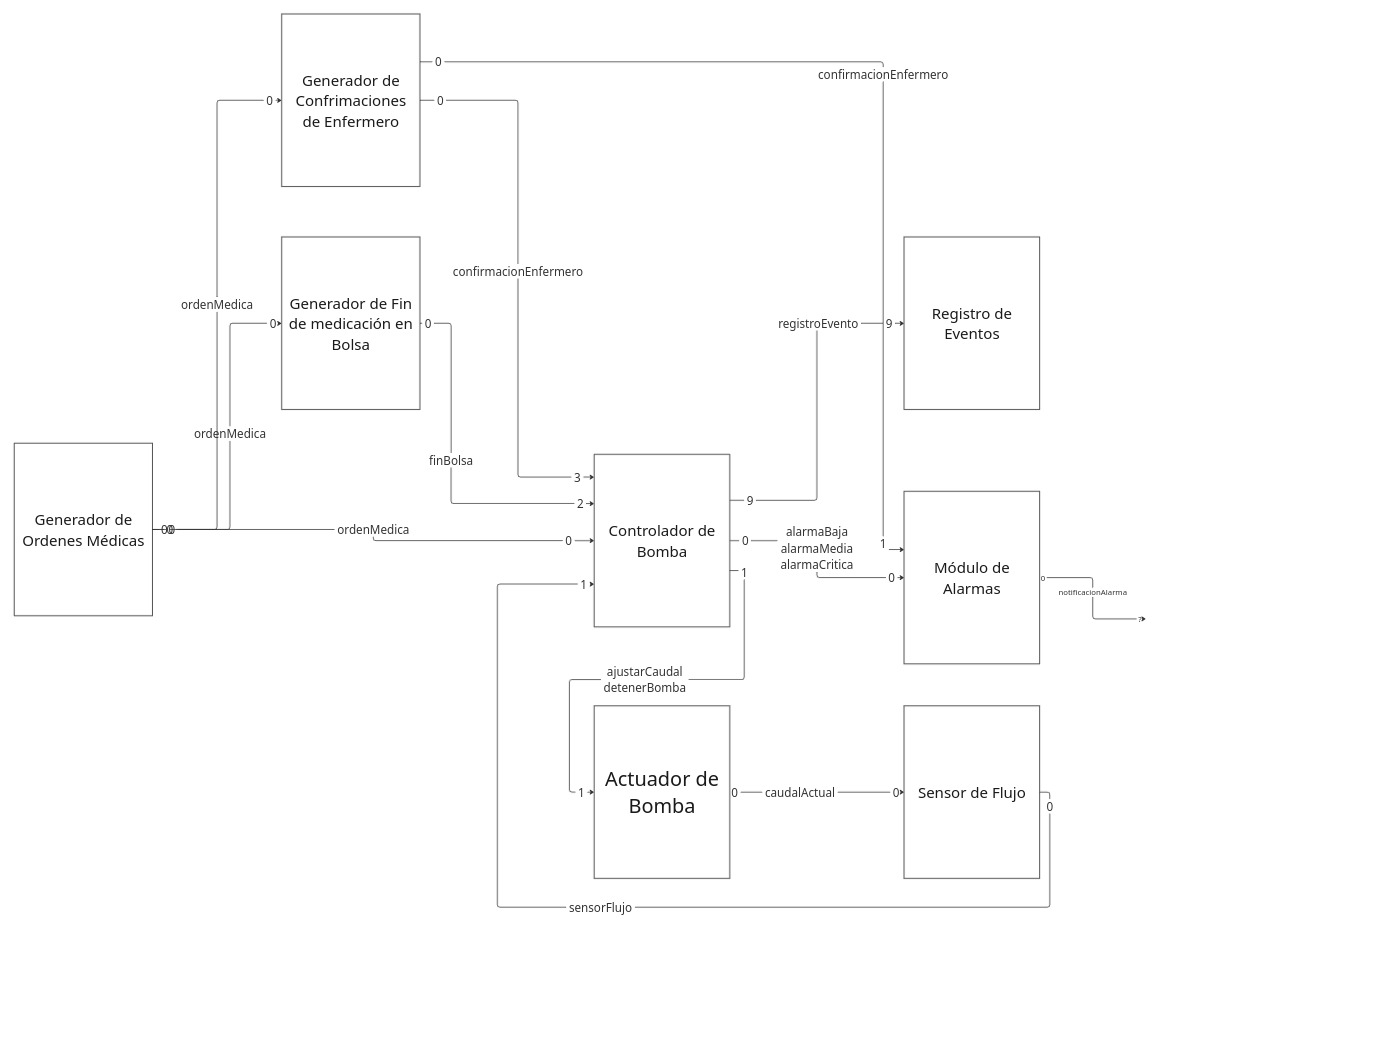
\includegraphics[width=1.2\textwidth]{devs_version_5.jpg} 
    \caption{Diagrama de acoplamiento del sistema de bomba de infusión.}
    \label{fig:mi_imagen}
\end{figure}


\end{document}
